\section{Vorbereitung}
\textbf{Die Versuchsvorbereitung ist Bestandteil des Versuchs. Sie erhalten dafür ein gesondertes Testat.\\
Ohne testierte Vorbereitung können Sie den Versuch nicht durchführen.}\\
\begin{enumerate}[label=\alph*)]
  \item Für die Versuchsdurchführung verwenden Sie das im Labortisch eingebaute Netzmodell nach Abbildung ~\ref{img2.1.1}. Skizzieren Sie eine Schaltung zur Bestimmung der Netzform (siehe Aufgabe 3.1) 
    \begin{figure}[h!]
      \begin{center}
        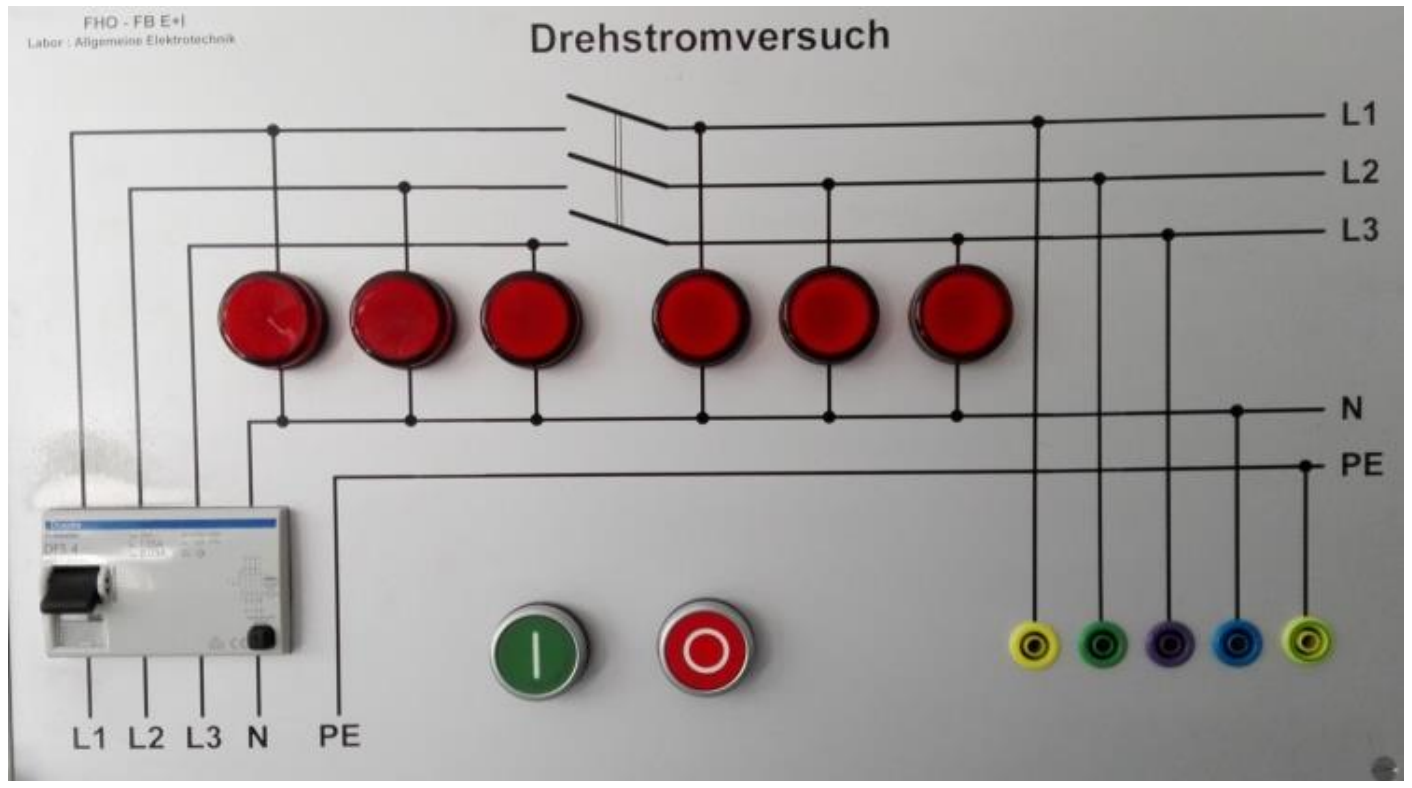
\includegraphics[width=0.5\textwidth]{img/img2.1.1.png}
      \end{center}
      \caption{Netzmodell am Versuchstisch }\label{img2.1.1}
    \end{figure}
    
  \item Skizzieren Sie eine Schaltung zur Bestimmung des Fehlerstromes des FI-Schutzschalters mit Hilfe des FI-Testers aus Abbildung \ref{img2.2.1} und Multimetern zur Strom- bzw. Spannungsmessung. 
	\begin{figure}[h!]
		\centering
		\begin{subfigure}[b]{0.41\textwidth}
			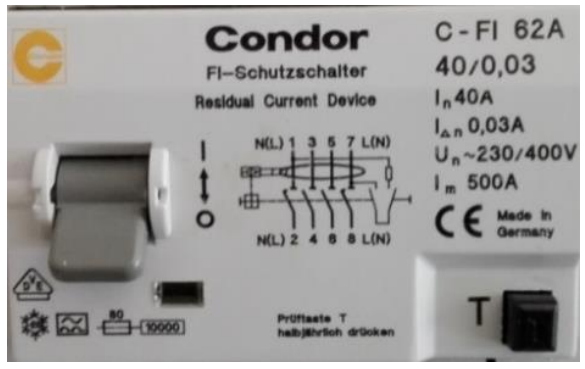
\includegraphics
			[width=\textwidth]{img/img2.2.1.png}
		\end{subfigure}\hfil
		\begin{subfigure}[b]{0.49\textwidth}
		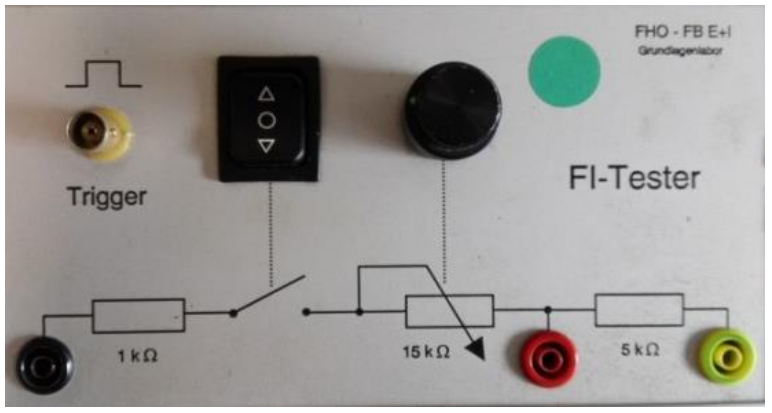
\includegraphics
		[width=\textwidth]{img/img2.2.2.png}
		\end{subfigure}
	\caption{FI-Schutzschalter und FI-Tester}\label{img2.2.1}
	\end{figure}
	
	Der FI-Tester wird an einen Außenleiter und den Neutralleiter angeschlossen. Im Tester sind drei Widerstände in Reihe geschaltet: $R_{1}=1k\Omega$ , $R_{var}=0\textohm - 15k\Omega$ und ein weiterer Widerstand von $R_{2}=5k\Omega$. Der $5k\Omega$-Widerstand wird nicht für den Versuch verwendet.\\

	\begin{figure}[h!]
		\begin{center}
			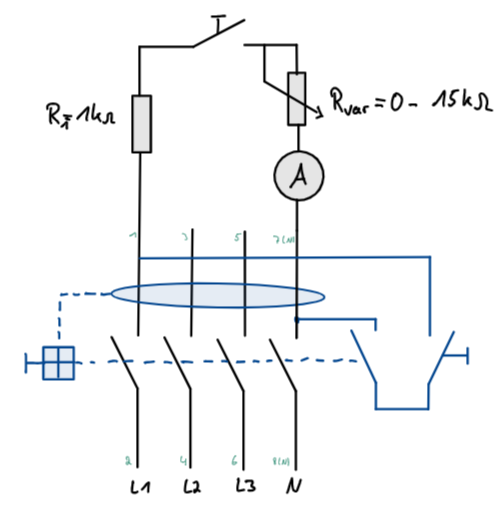
\includegraphics[width=0.5\textwidth]{img/img2.2.3.png}
		\end{center}
		\caption{Fehlerstrommessung am FI-Schutzschalter mit FI-Tester und Multimetern}\label{img2.2.3}
	\end{figure}
  \pagebreak
	

	% {
	% % \renewcommand{\abstractname}{Herleitung zum FI-Tester}
 %  \centering{Herleitung zum FI-Tester}\\\ \\
	% % % \begin{abstract}
	% 	\fcolorbox{black}{lightgray}{\parbox{\linewidth}{
	% 			\begin{align*}			
 %          I_{fehler}&=I_{ges}\cdot \frac{R_v+R_{var}}{R_{fehler}}\\ 
 %          I_{ges} &=\frac{U}{R_{ges}}\\ 
 %          I_{ges} &=\frac{U}{\frac{R_{fehler}\cdot(R_v+R_{var)}}{R_{fehler}+(R_v+R_{var})}}\\
 %          I_{ges} &={U}\cdot{\frac{R_{fehler}+R_v+R_{var}}{R_{fehler}\cdot(R_v+R_{var})}}\\
 %          I_{fehler}&={U}\cdot{\frac{R_{fehler}+R_v+R_{var}}{R_{fehler}\cdot(R_v+R_{var})}}\cdot \frac{R_v+R_{var}}{R_{fehler}}\\ 
 %          I_{fehler}&={U}\cdot{\frac{R_{fehler}+R_v+R_{var}}{(R_{fehler})^2}}\\
 %          I_{fehler}&={230\ V}\cdot{\frac{5\ k\Omega+1\ k\Omega+R_{var}}{(5\ k\Omega)^2}}\\
 %          I_{fehler}&={230\ V}\cdot{\frac{6\ k\Omega+R_{var}}{25\ (k\Omega)^2}}\\
 %          R_{var}&=\frac{I_{fehler}\cdot{25\ (k\Omega)^2}}{230\ V}-6\ k\Omega\\
 %          R_{var}&=\frac{15\ mA\cdot{25\ (k\Omega)^2}}{230\ V}-6\ k\Omega\\
	% 			\end{align*}
	% 		}}
	% % \end{abstract}
	% }
	
	Die Zielsetzung besteht darin, den FI-Schutzschalter auszulösen, sobald ein Differenzstrom von mehr als 30 mA auftritt. Daher müssen wir den variablen Widerstand von 0 Ohm solange verkleinern, bis der FI-Schalter auslöst.
\begin{align*}
  
\end{align*}
  \item An einem Vierleiter-Drehstromnetz ist eine symmetrische ohmsch-induktive Last (Reihenschaltung von Induktivität und Widerstand) in Sternschaltung angeschlossen. Bestimmen Sie formelmäßig die nötige Kapazität in Parallelschaltung (Sternschaltung), um eine vollständige Kompensation ($\cos \varphi = 1$) zu erreichen. 


  \item Bestimmen Sie formelmäßig die nötige Kapazität, wenn die Kondensatoren in Dreieck verschaltet sind.

  \item An einem Vierleiter-Drehstromnetz mit der konstanten Außenleiterspannung $U = 380\ V$ sind nach Abbildung \ref{img2.6.1} unsymmetrische Lasten angeschlossen. Bestimmen Sie rechnerisch und graphisch den Strom im Nullleiter, legen Sie dazu $\underline{U_1}$ in die reelle Achse, $f = 50\ Hz$!

\item Bestimmen Sie nun für dieselbe Last alle Ströme und Spannungen ohne angeschlossenen Neutralleiter. Zeichnen Sie das Zeigerdiagramm der Spannungen $\underline{U_{1K}},\ \underline{U_{2K}} \text{ und } \underline{U_{3K}}$. 
  \begin{figure}[h!]
    \begin{center}
      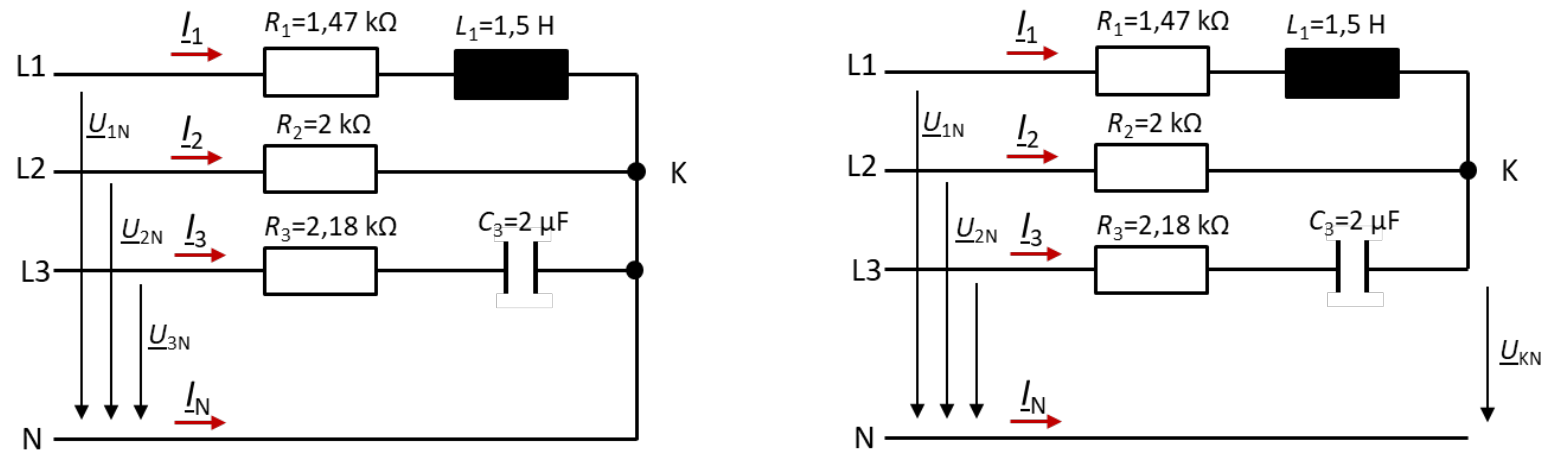
\includegraphics[width=0.95\textwidth]{img/img2.6.1.png}
    \end{center}
    \caption{Last a mit und ohne angeschlossenen Neutralleiter (Gruppe XXa)}\label{img2.6.1}
  \end{figure}
  
\end{enumerate}
